\documentclass[../diplomski_rad.tex]{subfiles}

\begin{document}

\sloppy

\justifying
U ovom radu razvijen je bežični nosivi sustav za praćenje distribucije tekućina u tijelu pomoću mjerenja bioimpedancije.
Blok shema sustava prikazana je na slici \ref{slk:blok_shema}.
Sustav se temelji na upotrebi STM32WB5MMG modula koji omogućava Bluetooth Low Energy (BLE) komunikaciju. 
Ključne komponente sustava uključuju MAX30009 senzor za mjerenje bioimpedancije, 
BME280 senzor za mjerenje temperature i ISM330DHCX senzor za mjerenje ubrzanja. 
Izmjereni podaci se putem BLE veze šalju ispitnom okruženju, omogućujući kontinuirano praćenje i analizu 
fizioloških parametara korisnika. 

\begin{figure}[htb]
    \centering
    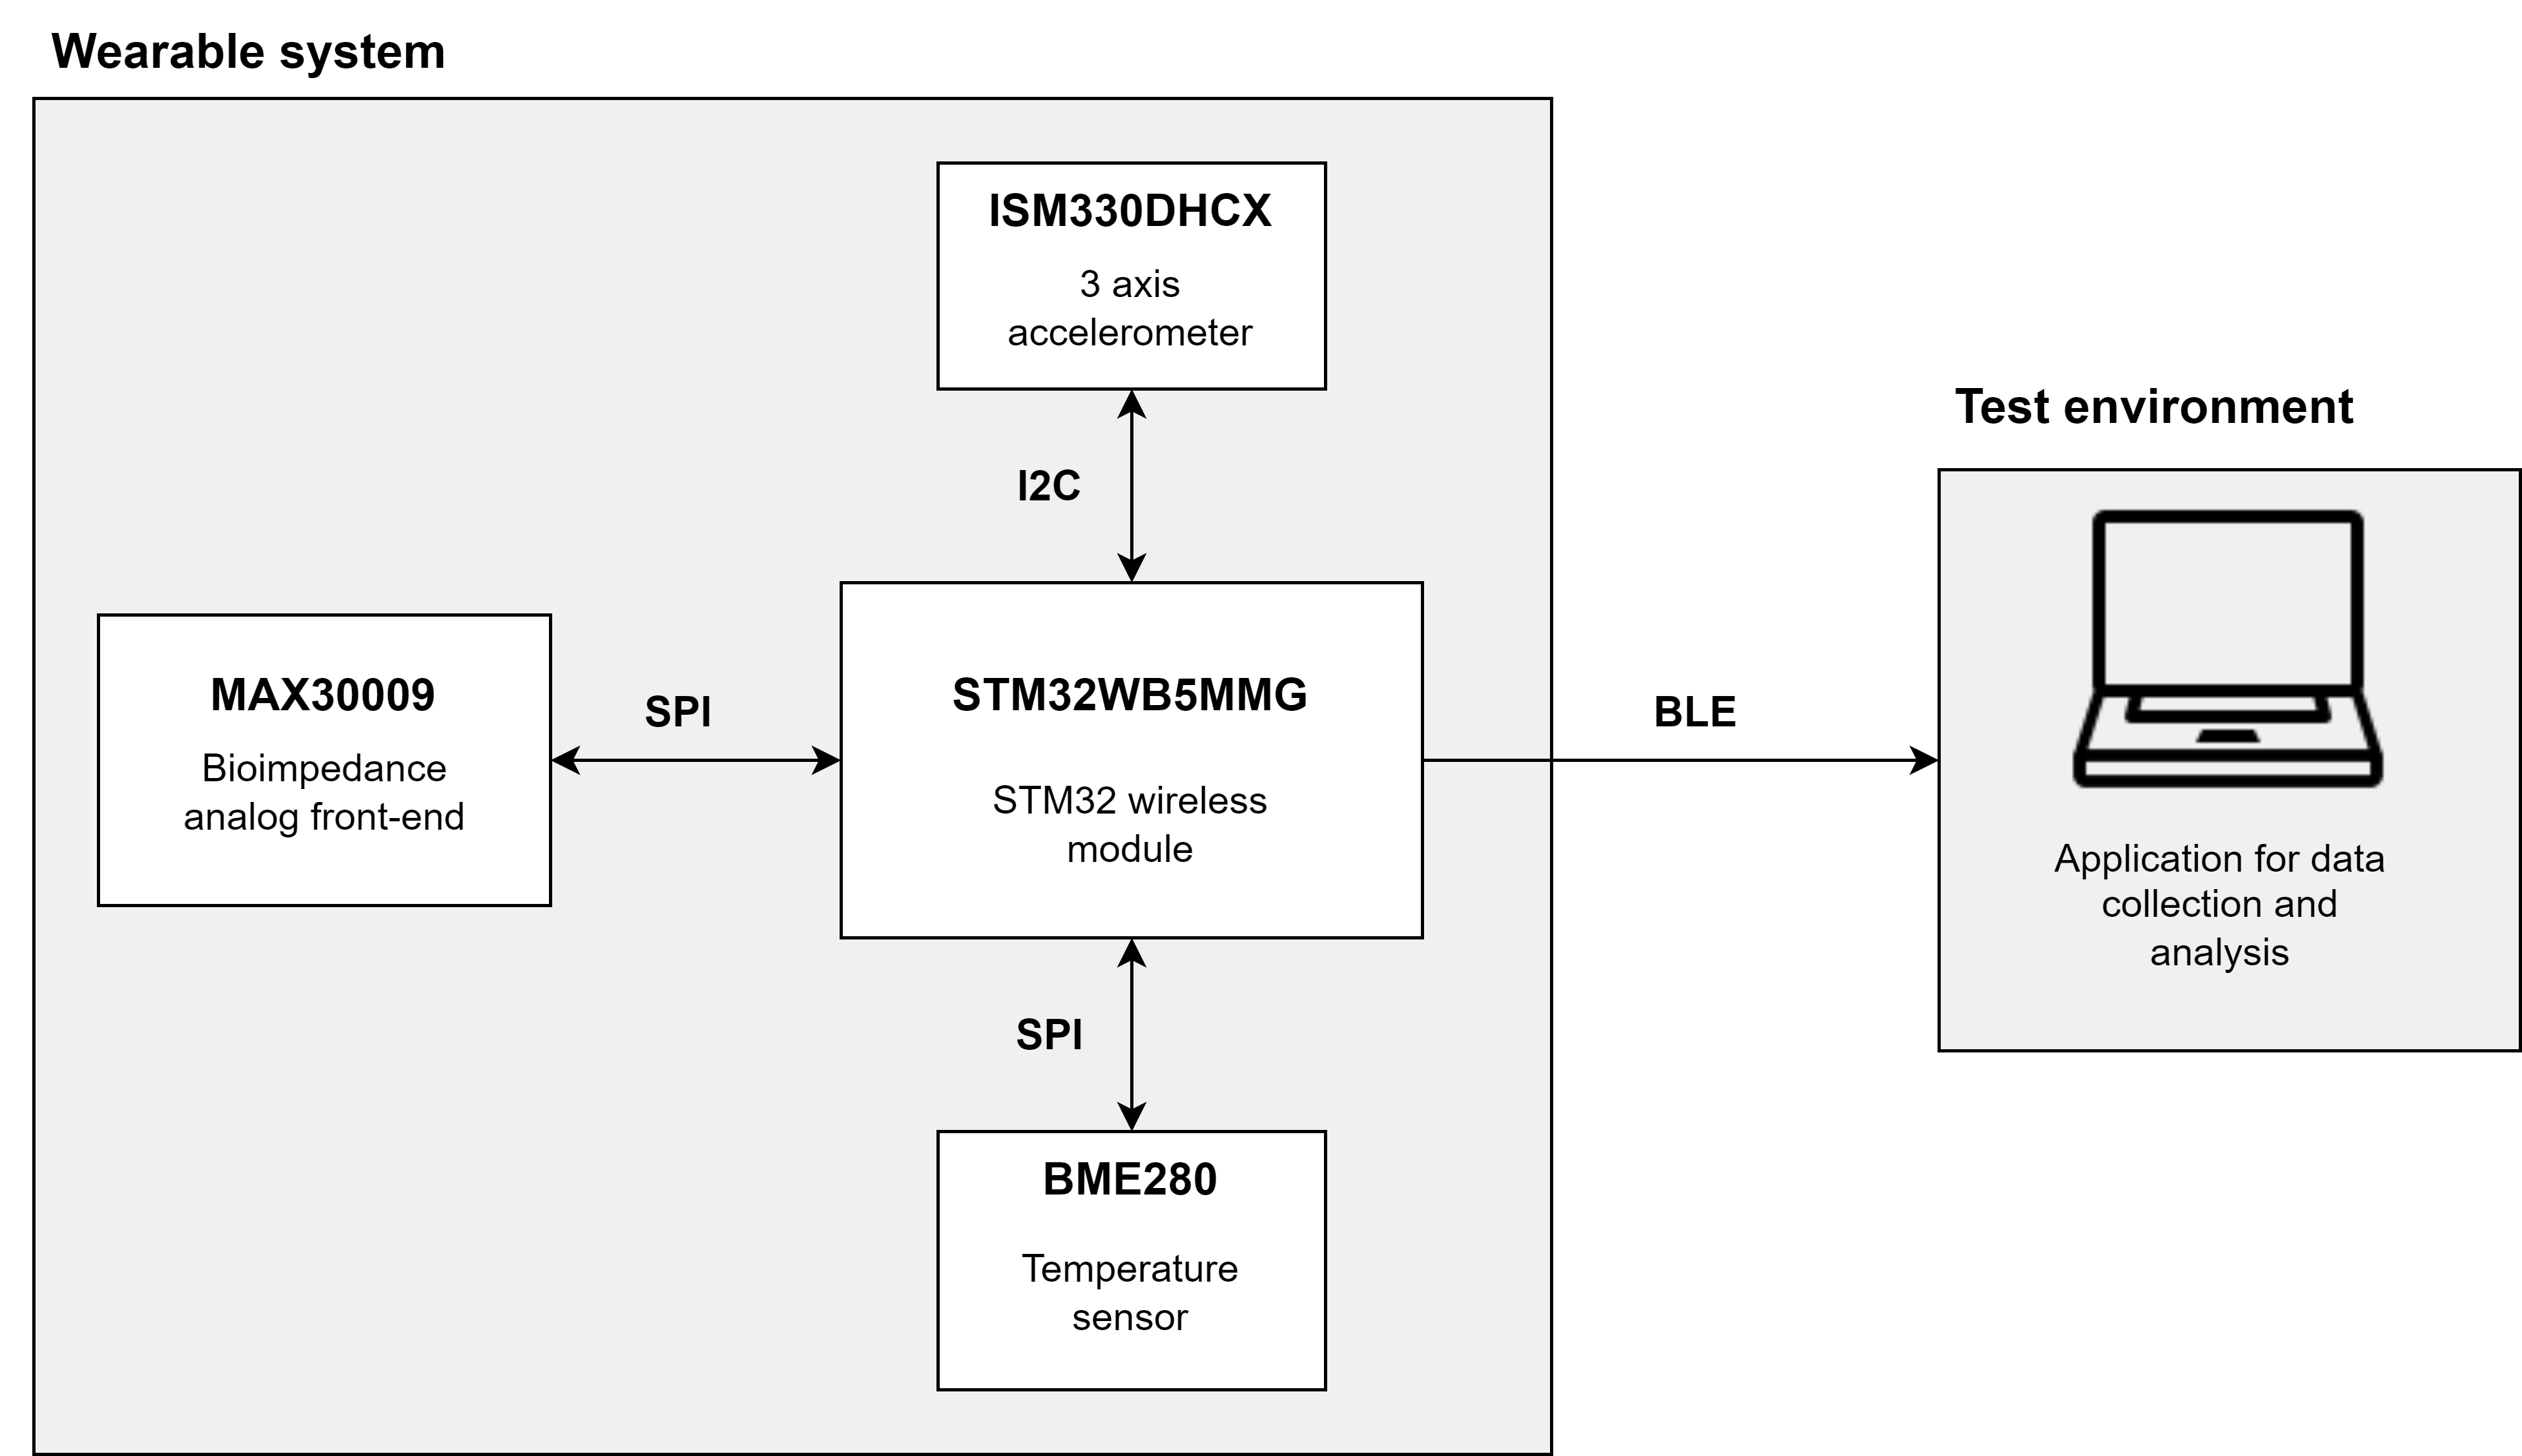
\includegraphics[width=1\textwidth]{Figures/shema_sustava.png} 
    \caption{Block shema razvijenog sustava}
    \label{slk:blok_shema}
\end{figure}

U tekstu koji slijedi opisani su svi korišteni elementi sustava.

\section{STM32WB5MMG bežični modul}

STM32WB5MMG bežični modul predstavlja kompaktno i visoko integrirano rješenje za razvoj pametnih uređaja koji zahtijevaju bežičnu povezanost. 
Baziran je na mikrokontroleru STM32WB55VGY te pruža mogućnost Bluetooth Low Energy i Zigbee bežične komunikacije. 
U modul je integrirana antena i kvarcni oscilatori što znatno olakšava i ubrzava razvoj sklopovlja.  

\begin{figure}[htb]
    \centering
    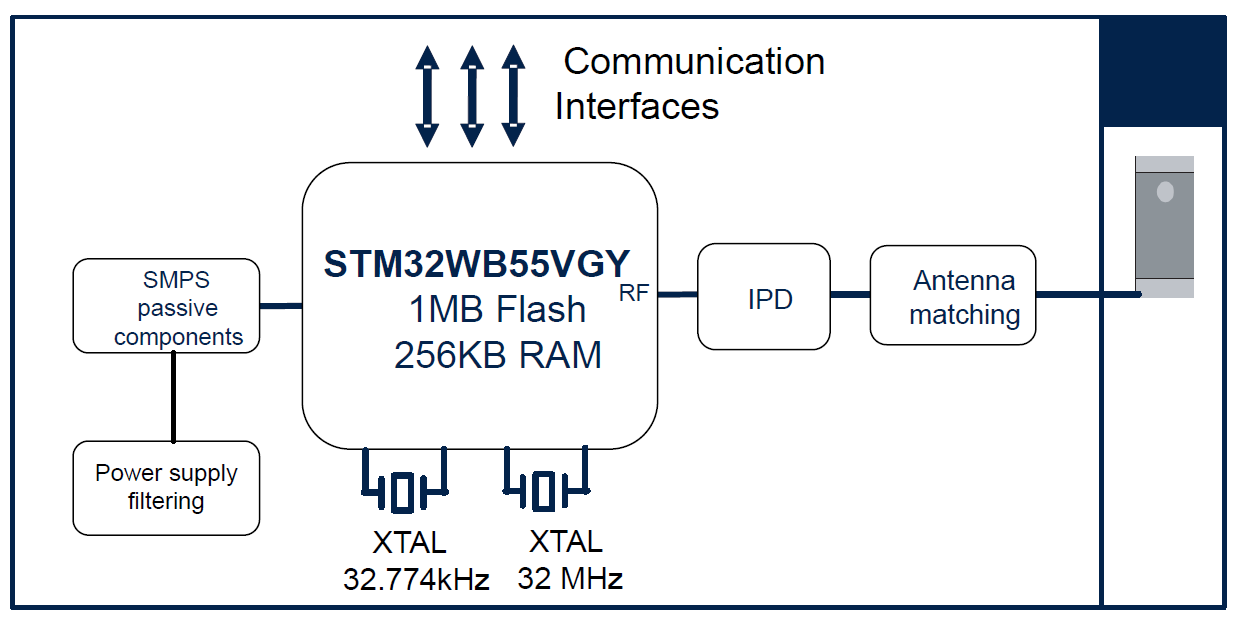
\includegraphics[width=0.75\textwidth]{Figures/stm32module.png} 
    \caption{Block shema STM32WB5MMG modula \cite{stm32module}}
    \label{slk:stm32module}
\end{figure}

Modul dolazi u LGA kućištu veličine 7.3x11 milimetara prikazanom na slici \ref{slk:stm32module_kuciste}. 
Iz blok sheme modula, prikazane na slici \ref{slk:stm32module}, 
vidljivo je kako se modul sastoji od:
\begin{itemize}
    \item STM32WB55VGY mikrokontrolera,
    \item antene,
    \item niskofrekvencijskog kvarcnog oscilatora frekvencije 32.768 kHz,
    \item visokofrekvencijskog kvarcnog oscilatora frekvencije 32 MHz,
    \item Pasivne komponente za SMPS (engl. \textit{switched-mode power supply}) 
    \item Integrirane pasivne komponente (IPD) za uklanjanje harmonika i usklađivanje RF impedancije.     
  \end{itemize} 
Zbog niske potrošnje, visokog stupnja integriranosti i malih dimenzija pogodan je za razvoj nosivih uređaja, 
čija je glavna karakteristika da moraju biti bežično povezani sa drugim uređajima. 

\begin{figure}[htb]
    \centering
    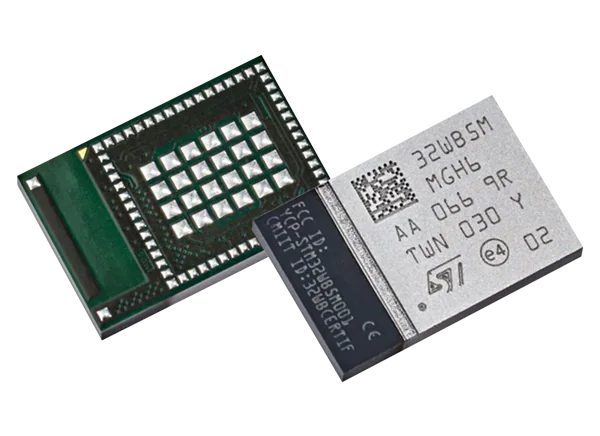
\includegraphics[width=0.75\textwidth]{Figures/modul.png} 
    \caption{Kučište STM32WB5MMG modula \cite{modul_slika}}
    \label{slk:stm32module_kuciste}
\end{figure}

\subsection{STM32WB55VGY mikrokontroler}

STM32WB55VGY je dvojezgreni mikrokontroler s ugrađenom podrškom za bežičnu komunikaciju. 
To je sistem na čipu koji unutar jednog čipa integrira mikrokontroler opće namjene i mrežnu funcionalnost. 
Sastoji se od dvije jezgre, ARM Cortex-M4 te ARM Cortex-M0+.  
ARM Cortex-M4 jezgra izvršava aplikacijski kod te radi na maksimalnoj frekvenciji od 64 MHz. 
Mrežni procesor ARM Cortex-M0+ zadužen je za upravljanje bežičnim komunikacijskim protokolima 
te potpuno neovisno od aplikacijske jezgre održava bežičnu vezu.
Jezgre međusobno komuniciraju pomoću međuprocesorskog komunikacijskog kontrolera (engl. \textit{IPCC,  Inter Processor
Communication Controller}). 
Dijeljenje resursa među jezgrama kontrolirano je sklopovskim semaforima.

\begin{figure}[htb!]
    \centering
    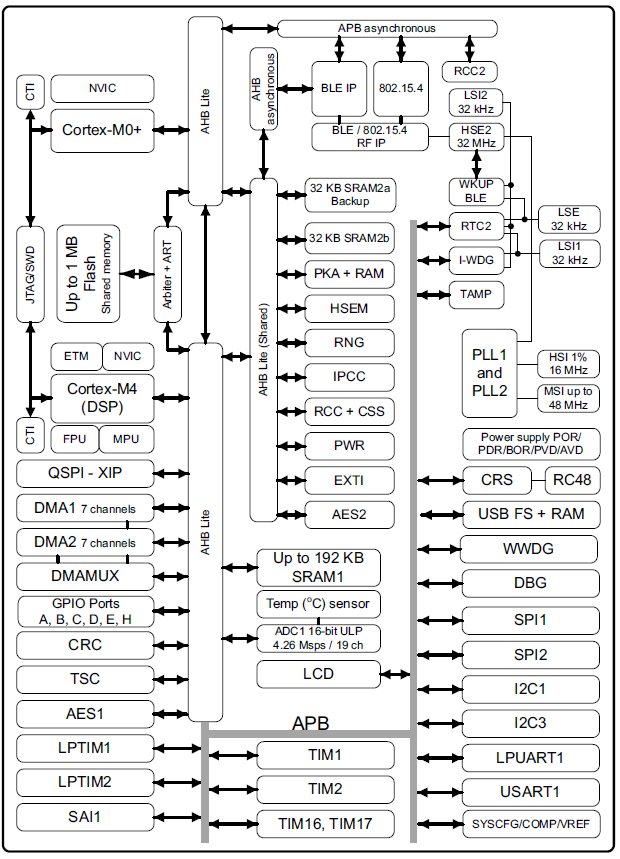
\includegraphics[width=0.6\textwidth]{Figures/stm32mikro.png} 
    \caption{Block shema STM32WB55VGY mikrokontrolera \cite{stm32mikro}}
    \label{slk:stm32mikro}
\end{figure}

Mikrokontroler ima 1MB flash memorije, 256kB SRAM memorije te sve uobičajne periferije za mikrokontrolere opće namjene. 
Na slici \ref{slk:stm32mikro} prikazana je blok shema mikrokontrolera na kojoj su vidljive sve dostupne periferije.
Razvoj programske potpore za korišteni mikrokontroler opisan je u poglavlju (\ref{chap:programska_podrska}).

\section{Senzorski sustavi}

Senzori su ključan dio razvijenog nosivog sustava jer omogućuju kontinuirano praćenje podataka potrebnih 
za dijagnostiku i praćenje zdravstvenog stanja pacijenata u stvarnom vremenu.
U daljnjem tekstu dan je detaljan pregled svih korištenih senzora razvijenog sustava.

\subsection{MAX30009 integrirano sučelje za mjerenje bioimpedancije}

MAX30009 je integrirano sučelje za mjerenje bioimpedancije dizajnirano za primjene u nosivim tehnologijama. 
Izrazito je male potrošnje (250 $\mu$W na napajanju od 1.8 V) \cite{max30009} i malih dimenzija (2.03x2.03 mm) što ga čini idealnim izborom za bežični nosivi uređaj.  

Senzor radi na principu puštanja sinusne struje kroz tijelo i mjerenjem nastalog pada napona kroz tijelo. 
U sebi ima integrirani generator pobudne sinusne struje u širokom rasponu frekvencija i jakosti struja. 
Raspon frekvencija je od 16 Hz do 500 kHz, a jakosti struja od 16nA\textsubscript{RMS} do 1.28mA\textsubscript{RMS} \cite{max30009}.
Uzbudna struja stvara se sklopom za direktnu digitalnu sintezu (engl. \textit{Direct Digital Synthesis, DSS}). 
DDS sklop služi za generiranje preciznih sinusnih signala uz mogućnost brzog podešavanja frekvencije.  

Ulazni priključci elektroda spojeni su na multipleksore čime se dobiva mogućnost izbora 
između različitih setova elektroda. Također senzor podržava dvožično kao i četverožično mjerenje bioimpedancije.

\begin{figure}[htb]
    \centering
    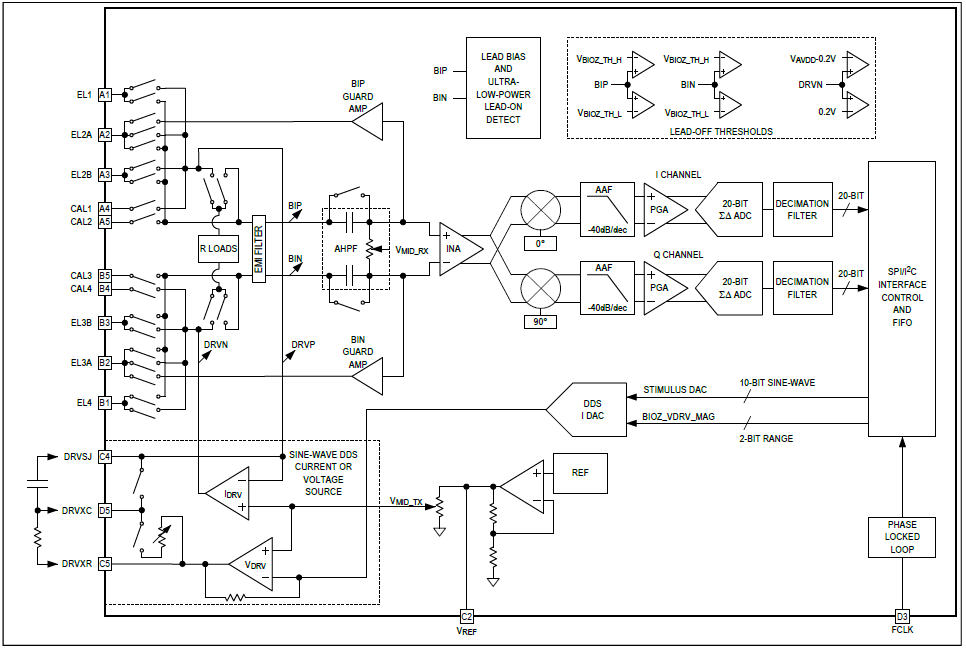
\includegraphics[width=1\textwidth]{Figures/max30009_bioz.png} 
    \caption{Block shema MAX30009 integriranog sučelja za mjerenje bioimpedancije \cite{max30009_datasheet}}
    \label{slk:max30009_bioz}
\end{figure}

Kako bi se iz izmjerenog napona dobila amplituda i faza bioimpedancije koristi se I/Q (engl. \textit{In-phase/Quadrature}) 
demodulator prikazan na slici \ref{slk:max30009_receive}. 
\textit{In-phase} grana dobiva se množenjem sinusnog napona sa pravokutnim signalom jednake faze i frekvencije kao pobudna struja.
U slušaju \textit{Quadrature} grane pravokutnom signalu se dodaje zakašnjenje u fazi od 90 stupnjeva.  
Pravokutni signal može se prikazati Fourierovim redom, no kako je prikazano na slici \ref{slk:max30009_demodulator}, 
nakon prolaska signala kroz niskopropusne filtre ostaje samo istosmjerna komponenta. 
Na ovaj način početni sinusni signal je rastavljen na zbroj sinusa i kosinusa iste frekvencije, ali različitih amplituda koje su 
konačni izlaz demodulatora.

\begin{figure}[htb]
    \centering
    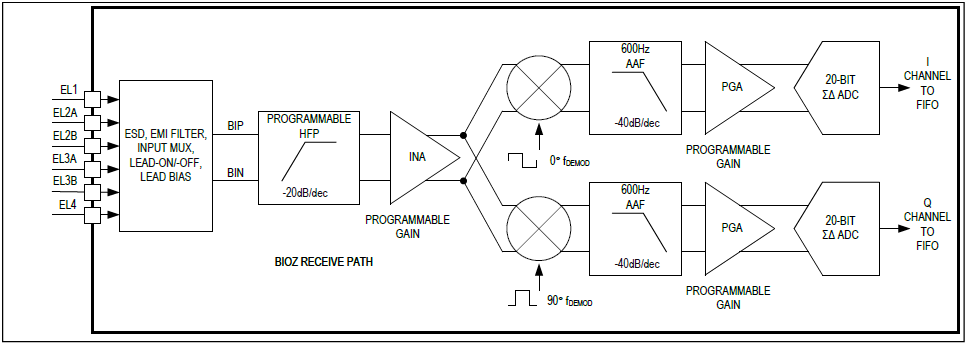
\includegraphics[width=1\textwidth]{Figures/max30009_receive.png} 
    \caption{Block shema demodulatora \cite{max30009_datasheet}}
    \label{slk:max30009_receive}
\end{figure}

Poznavajući DC vrijednosti I i Q grana na izlazu demodulatora moguće je izračunati amplitudu i fazu mjerene impedancije.
Ako sa $U_{I,DC}$ i $U_{Q,DC}$ označimo vrijednosti I i Q grane dobivene na izlazu demodulatora, 
sljedeće jednadžbe nam daju vrijednost amplitude i faze impedancije:
\begin{equation}
    \label{jed:cpe}
    \theta = arctg(\frac{U_{Q,DC}}{U_{I,DC}})
\end{equation} 
\begin{equation}
    \label{jed:cpe}
    Z = K\sqrt{U_{I,DC}^2+U_{Q,DC}^2}
\end{equation} 
Kako amplitude lokalnih pravokutnih oscilacija nisu poznate rezultat mjerenja potrebno je pomnožiti sa kalibracijskom 
konstantom \textit{K}. Na početku rada sustava potrebno je izvršiti kalibraciju mjerenjem otpornika poznatog iznosa i 
izračunavanjem korekcijske konstante. Postupak je potrebno provesti zasebno za svaku frekvenciju rada sustava.

MAX30009 pruža kalibracijski priključak za vanjski četverožičani precizni referentni otpor koji se koristi tijekom kalibracije. 
Također, dostupni su i interni programabilni otpornici koji se mogu koristit za kalibraciju, ali uz manju točnost od vanjskog referentnog otpornika.
Kalibracija je potrebna prilikom korištenja MAX30009 za bioimpedancijska mjerenja koja zahtijevaju apsolutnu točnost poput BIA i BIS mjerenja.

\begin{figure}[htb]
    \centering
    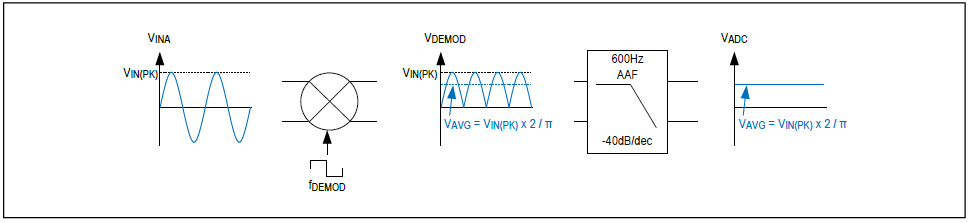
\includegraphics[width=1\textwidth]{Figures/max30009_demodulator.png} 
    \caption{Postupak demodulacije sinusnog napona \cite{max30009_datasheet}}
    \label{slk:max30009_demodulator}
\end{figure}

Sustav se konfigurira pomoću 8 bitnih softverskih registara, a izlazni podatci pohranjuju se u 
FIFO (engl. \textit{First In First Out}) spremnik veličine 256 uzoraka.
FIFO spremnik je struktura za pohranu podataka u kojoj se podatci čitaju onim redosljedom kojim su u strukturu i pisani. 
Svaki očitani uzorak u FIFO spremnik pohranjuje se u 3 bajta i sastoji se od identifikacijske oznake veličine 4 bita te vrijednosti očitane s ADC 
pretvornika veličine 20 bitova. 
Oznaka razlikuje podatke očitane s I grane od onih očitanih s Q grane.
Vrijednosti očitane s ADC pretvornika zapisane su u dvojnom komplementu. 
Sustav je moguće konfigurirati na način da generira prekid mikrokontroleru kada se FIFO napuni s određenim brojem uzoraka. 
Broj uzoraka kod kojeg će se prekid generirati određuje se konfiguracijskim konstantama. Na osnovu nastalog prekida 
mikrokontroler tada čita dostupne podatke iz FIFO spremnika čime se spremnik automatski prazni.  

\subsection{Temperaturni senzor}

BME280 senzor je visokoprecizni, višenamjenski senzor koji omogućava mjerenje temperature, 
relativne vlažnosti i atmosferskog tlaka. 
Ovaj senzor, razvijen od strane kompanije Bosch Sensortec, poznat je po svojoj visokoj točnosti i 
niskoj potrošnji energije, što ga čini idealnim za primjenu u nosivim uređajima i IoT rješenjima.

BME280 omogućuje precizna očitanja s minimalnim odstupanjima. 
Senzor može mjeriti temperaturu u rasponu od -40°C do 85°C s točnošću od ±0.5°C, 
relativnu vlažnost u rasponu od 0\% do 100\% s točnošću od ±3\%, te atmosferski tlak u 
rasponu od 300 hPa do 1100 hPa s točnošću od ±1 hPa \cite{bme280_datasheet}.

\begin{figure}[htb]
    \centering
    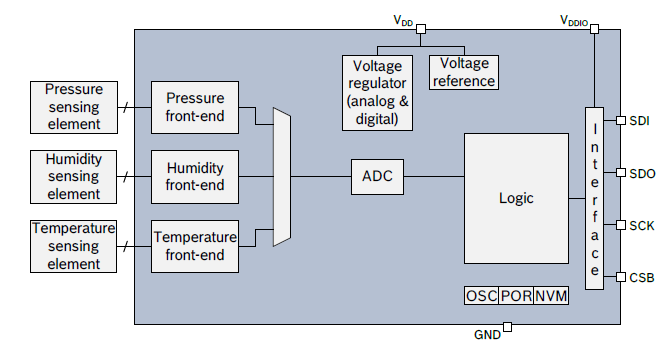
\includegraphics[width=1\textwidth]{Figures/bme280.png} 
    \caption{Blok shema senzora BME280\cite{bme280_datasheet}}
    \label{slk:shema_bme280}
\end{figure}

- jedna pametna o tome sta ce to u ovom sustavu

%Integracija BME280 senzora u sustav omogućava kontinuirano praćenje okolišnih uvjeta, 
%što je ključno za točne i pouzdane rezultate mjerenja bioimpedancije. 
%Na primjer, promjene u temperaturi i vlažnosti mogu utjecati na bioelektrična svojstva kože, 
%te stoga uzimanje tih parametara u obzir omogućava bolju kalibraciju i interpretaciju podataka.

\subsection{Senzor inercije}

- promjeni tu senzor na ISM330DHCX

Senzor ICM-20948 koristi se za mjerenje inercije te pruža precizno praćenje kretanja i orijentacije u prostoru.
Unutar jednog čipa ima integriran akcelerometar, žiroskop i magnetometar što pruža sveobuhvatnu sliku o kretanju 
i položaju objekta u trodiomenzionalnom prostoru. 

- treba li tu sto detaljnije (komunikacjski protokoli, konkretne karakteristike..)?

\begin{figure}[htb]
    \centering
    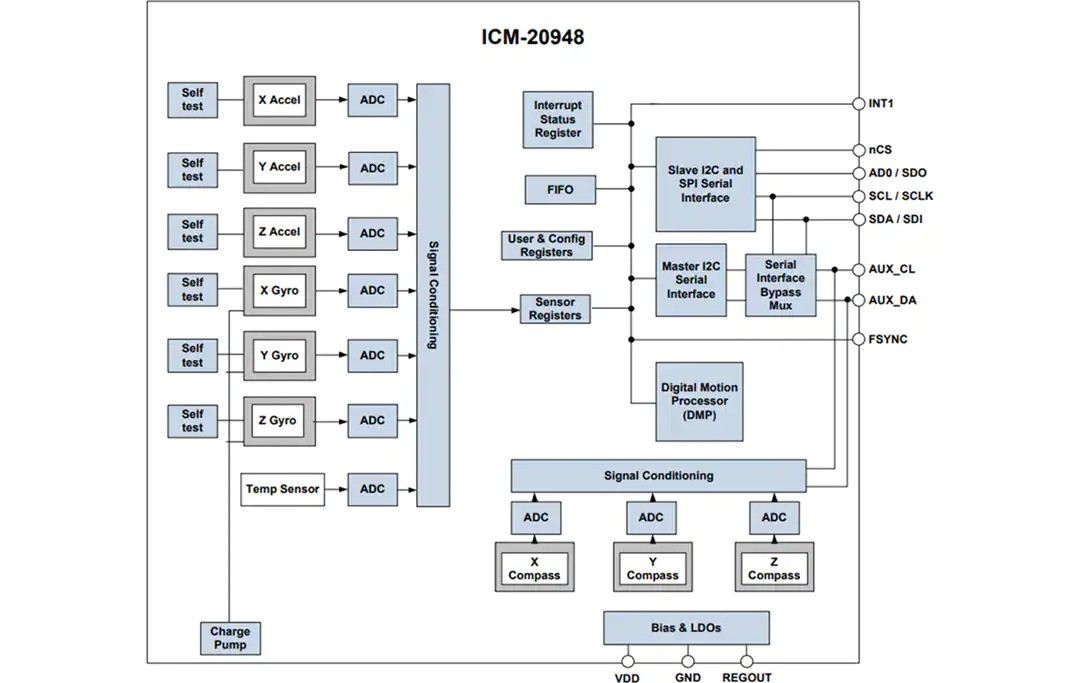
\includegraphics[width=0.75\textwidth]{Figures/ICM-20948.jpg} 
    \caption{Block shema senzora ICM-20948 \cite{icm20948}}
    \label{slk:icm20948}
\end{figure}

Senzor komunicira s ostatkom sustava pomoću I2C ili SPI komunikacije te na zahtjev šalje mikrokontroleru tražene podatke.
Važno je naglasiti da je ICM-20948 dizajniran s naglaskom na energetsku učinkovitost i malu potrošnju energije 
što ga čini dobrim izborom za nosive uređaje.

\end{document}